% Sample file on how to use subfiles.
\documentclass[ExampleMasters.tex]{subfiles}

\begin{document}

\chapter{Vehicle Model}

\lipsum 
A layout of the entire model architecture is as shown in Figure (\ref{fig:architecture}). This section will cover a description of the cycle , driver and vehicle model. \\

\begin{figure}[ht!]
	\begin{center}
		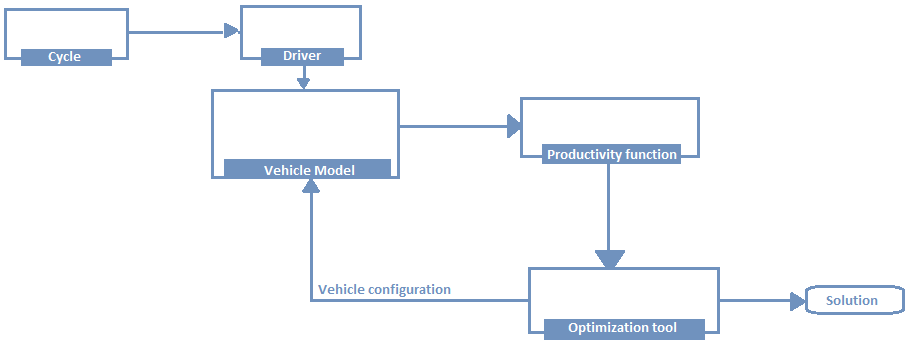
\includegraphics[width=0.75\textwidth]{figures/VehicleModel/architecture2.png}
	\end{center}
	\caption{Model architecture - Overview}
	\label{fig:architecture}
\end{figure}

\section{Driving Cycle}
\label{sec:drivingcycle}
The aim of the project is to find the most productive vehicle combination for a particular route. The route chosen for this is the 294 km E20/E6 highway from G\"oteborg to Malm\"o. This particular journey back and forth is quite popular among companies transporting goods and any findings of the report will be of key interest. 
The driving cycle data provided was recorded with a frequency of 1 Hz from an on-board GPS and it included:
\begin{itemize}
\item X-axis position data
\item Y-axis position data
\item Z-axis position data
\item Velocity
\item Distance covered
\end{itemize}

The inputs that are required from the driving cycle are the information of road gradient, instantaneous velocity and acceleration. Each of which could have been directly used from the provided data. However on subsequent study the speed signal was found to have considerable noise and many data points missing, making it unusable. The distance signal did not correspond to the distance covered as calculated from the position signal according to the equation below.

\begin{equation} \label{eq:cycle distance}
Distance = \sqrt{(x_{i+1} - x_i)^2 +(y_{i+1} - y_i)^2}
\end{equation}

This left only the position signals which had some issues that posed problems at first. The data is used to obtain the values of the slope of the road along the z axis (? Road gradient) since the vehicle model is represented as a one-track bicycle model and lateral effects are neglected. This is done as 

\begin{equation} \label{eq:cycle slope}
Slope =\frac{\delta Height}{\delta Distance} = \frac{z_{i+1} - z_i}{\sqrt{(x_{i+1}-x_i)^2 +(y_{i+1}-y_i)^2  }}
\end{equation}

The resolution of the position data was determined to be too low which caused problems when the slope was calculated as there were sudden big jumps in the slope values.

\begin{figure}[hb]
	\begin{center}
		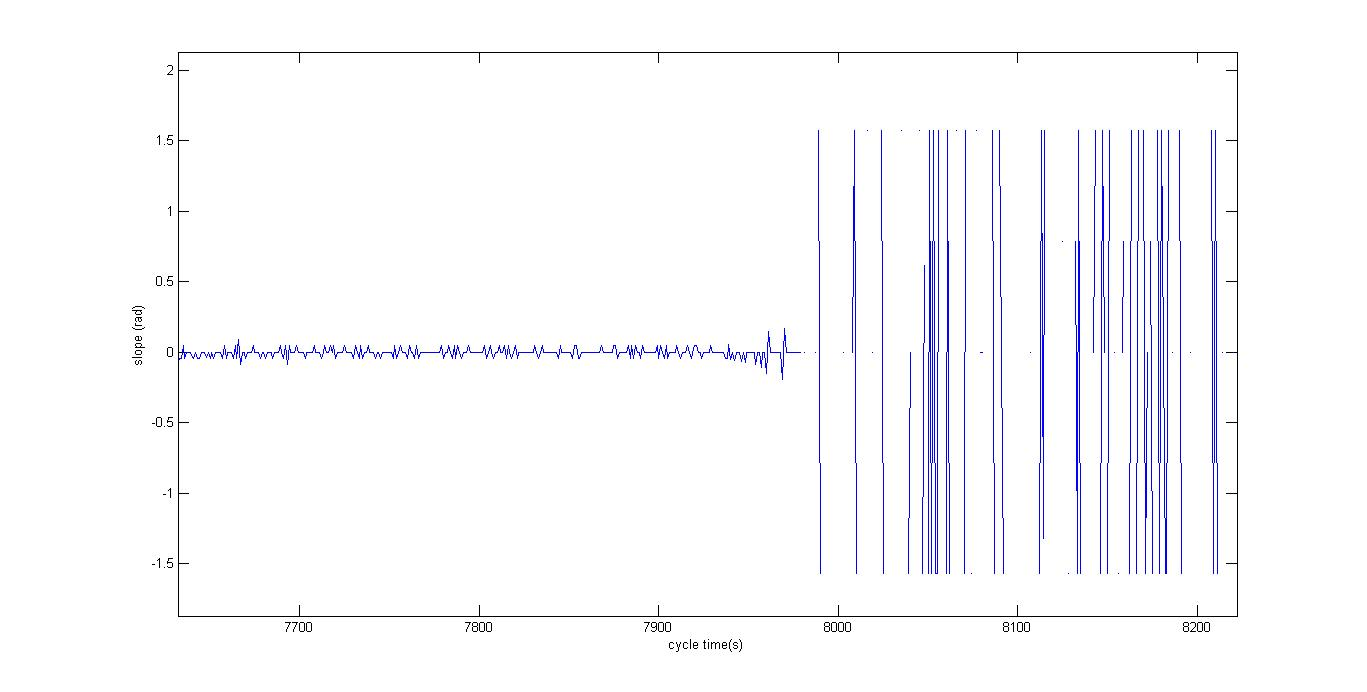
\includegraphics[width=0.75\textwidth]{figures/VehicleModel/noise.jpg}
	\end{center}
	\caption{Noisy slope signal.}
	\label{fig:noise}
\end{figure}

The data was also inconsistent resulting in a much disrupted slope signal as can be seen in figure (\ref{fig:noise}).This was addressed by introducing a rolling average filter for the position data along each axis. This approximates the value of the position over a range of old data to the average value in that range. The size of the range is dependent on the speed of the truck (i.e. taking a small sample size when the truck is moving faster and vice-versa) in order to provide a more realistic new signal. The sampling range was 10 above a threshold speed of 40 kmph and 5 for speeds below. When the position signals were filtered the slope was recalculated using equation (\ref{eq:cycle slope}). This gave an improved new slope data (data 2) as shown in figure(\ref{fig:rollingavg}).

\begin{figure}
	\begin{center}
		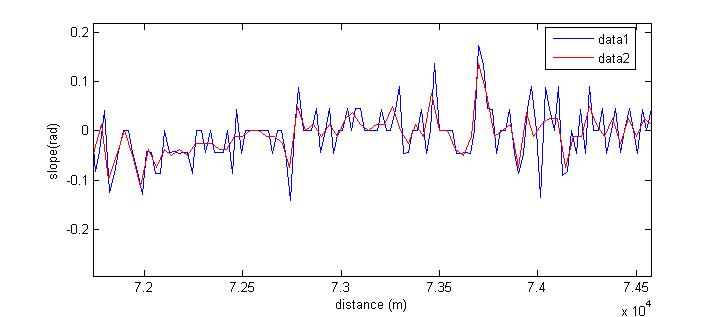
\includegraphics[width=0.75\textwidth]{figures/VehicleModel/rollingavg.jpg}
	\end{center}
	\caption{Slope signal after rolling average.}
	\label{fig:rollingavg}
\end{figure}

While the slope signal was now less irregular with a sampling frequency of 1 Hz the calculated slope was still too noisy to be used directly. To ensure the signal was smoother, a Matlab cubic spline function was used with a tuning factor of 0.1.Lastly the slope signal was redefined as against distance rather than time to suit the functionality of the driver model which is explained in more detail in Section  \ref{sec:drivermodel}.

\begin{figure}
	\begin{center}
		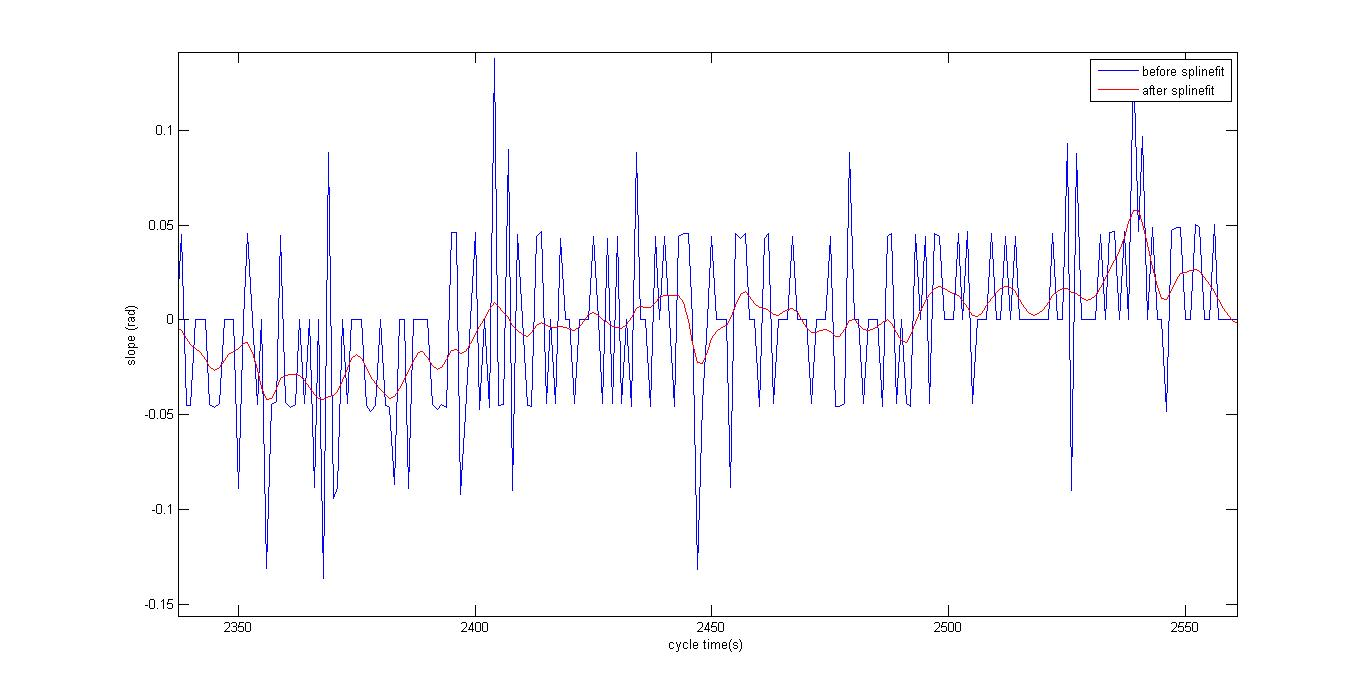
\includegraphics[width=0.75\textwidth]{figures/VehicleModel/aftersplinefit.jpg}
	\end{center}
	\caption{Slope signal after splinefit.}
	\label{fig:aftersplinefit}
\end{figure}

\section{Vehicle Model}
\label{sec:vehiclemodel}
The slope data is defined as against distance as the vehicles current position is calculated at each instant and the slope for that position is interpolated using the data. The slope information along with the vehicle parameters are used to calculate the total road resistive force as according to the equations %\ref{eq:roadresforce}% . 
The road resistive force consists of three main components: the slope force caused by the gradient of the road, the rolling force to overcome the road resistance and the aerodynamic force to counter the air drag.

\begin{equation} \label{eq:roadresforce}
Total road resistive force(F_{res}) =Slope force + Rolling force + Aerodynamic force
\end{equation}

\begin{equation} \label{eq:slopeforce}
Slope force=Equivalent combination weight(W_{eq})* g * \sin(slope)
\end{equation}

\begin{equation} \label{eq:rollingforce}
Rolling force =Coeff_{rolling resistance})* W_{eq} * g
\end{equation}

\begin{equation} \label{eq:aeroforce}
Aerodynamic force = \frac{1}{2} * \rho_{air}*Coeff_{rdrag})* frontal area *( instantaneous speed)^2
\end{equation}

\begin{equation} \label{eq:rollingforce}
W_{eq} =Gross combination weight(W_{gc})+Total inertial mass(W_{total inertia})
\end{equation}

The inertial effects of rotation were taken into account through an equivalent mass addition $(W_{total inertia})$ as seen in equation (\ref{eq:totinertialmass}). The term is defined as: 

\begin{equation} \label{eq:totinertialmass}
W_{total inertia}  =  Tire inertial mass(W_{tire inertia} )+Axle inertial mass(W_{axle inertia} )+Propeller shaft inertial mass(W_{prop inertia})+Transmission inertia mass(W_{trans inertia})
\end{equation}

\begin{equation} \label{eq:tireinertia}
W_{tire inertia} =Inertia_{tire}*(\frac{1}{tire radius(r)})^2
\end{equation}

\begin{equation} \label{eq:axleinertia}
W_{axle inertia} =Inertia_{axle}*(\frac1r)^2
\end{equation}

\begin{equation} \label{eq:propinertia}
W_{prop inertia} =Inertia_{prop shaft}*(\frac{final drive ratio(f.d)}{r})^2
\end{equation}

\begin{equation} \label{eq:transinertia}
W_{trans inertia} =Inertia_{transmission}*(\frac{gear ratio*f.d}{r})^2
\end{equation}

Once the vehicle combination returns information of the total traction that could be achieved by the truck in a particular instant, it is used with $F_{res}$ to calculate the actual acceleration that is achieved.
 
\begin{equation} \label{eq:acclforce}
Achieved acceleration force=Total achieved tractive force-Total resistive force(F_res)
\end{equation} 

\begin{equation} \label{eq:acclinstant}
Instantaneous acceleration=\frac{Achieved acceleration force}{Gross combination weight}
\end{equation} 

Through the basic motion equations is used to determine the distance travelled and speed at the next instant taking a cycle frequency of 1Hz. This continues till the total distance is covered. 

The truck is modelled as a longitudinal bicycle model where the focus lies on meeting the traction demand as provided by the driver model. Once the overall traction demand for an instant is calculated this is checked against the maximum grip limit traction capability and if found to be greater, the value for traction request is limited to the latter. The traction is then distributed between the units which is handled by the EMS, the explanation for which is covered in Section 3.4. When a traction request is provided to the unit, it is checked against the maximum propulsive or regenerative capacity of the units as a whole. In order to determine this value which is a machine property varying with machine speed, the axle speed is set, which in-turn passes through the axle differential and machine gearbox and translates to the machine speed. Thus cumulative maximum positive or negative tractive capacity is then determined. If the traction request is found to be less than this value and if the buffer associated to the unit is within operable range (explained in greater detail in Section 3.4) then the traction request is divided equally between driven axles.

The axle has the final drive ratio(f.d) associated with it. It is used to gear down the wheel speeds to a gearbox shaft speed as according to equations (\ref{eq:axlespeedgearing}) \&  (\ref{eq:axletorquegearing})

\begin{equation} \label{eq:axlespeedgearing}
Angular speed before differential =Longitudinal wheel speed*\frac{60}{2*\pi*tire radius(r)}
\end{equation}
\begin{equation} \label{eq:axletorquegearing}
Torque before differential =Tractive force at wheels*\frac{r}{f.d} 
\end{equation}

 So when a traction demand passes down to an axle, clears the grip limitation check and passes past the axle differential, it is sent to the machine transmissions. The functionality associated at the transmission level is simply to encapsulate the gearing reduction effects so as to arrive at the machine torque and speed given the selected gear. The losses at the transmission are neglected. 

\begin{equation} \label{eq:transpeedgearing}
Angular machine speed =Angular speed before differential*Selected gear ratio
\end{equation}

\begin{equation} \label{eq:transtorquegearing}
Machine torque =\frac{Torque before differential}{Selected gear ratio}
\end{equation}

\subsection{Machine model}
\label{sec:machinemodel}

When the axle speed information is passed down to the transmission the gear is selected as described in Section \ref{sec:drivermodel}, the machine speed is then calculated as above and assigned to the machine. Once the machine speed is set the values of maximum propulsive torque and in the case of a motor, the maximum regenerative torque are identified for the current speed. This information is accessed at the unit level as mentioned earlier .The torque requests are checked against the maximum torque capabilities regardless of whether it is positive propulsion torque or in the case of an electric motor, negative regenerative torque. If it within acceptable limits the machine torque is set to the demand value. The machine power to be demanded from the associated buffer is then calculated as 

\begin{equation} \label{eq:machinepowerdem}
Power demand=Machine torque*MachineRPM*\frac{2*\pi}{60}
\end{equation}

\subsection{Buffer model}
\label{sec:machinemodel}

The fuel tank or the battery, depending on the machine, receives a power demand from the machine. This is also converted into an energy demand for that particular instant which is calculated by assuming that the power is constant for a fixed time interval which the whole cycle has been discretised into (1 second by default). The brake specific fuel consumpsion $(B.S.F.C.)$ of the engine for the particular point is determined by the machine and the data is provided to the fuel tank.  On receiving the power demand and B.S.F.C, the amount of fuel to be consumed from the fuel tank to provide the power is calculated for that instant as shown below.

\begin{equation} \label{eq:fueldem}
Instantaneous fuel demand=\frac{Instantaneous power demand(P_{dem}) * B.S.F.C * Time}{1000*\rho_{fuel}}
\end{equation}

When power is demanded from the battery, information of the operating efficiency of the machine $(\eta_{Machine})$  is also sent. This information is recieved from the machine as it depends on its instantaneous point of operation. The battery model does not account for variations in open circuit voltage(OCV) and battery efficiency with state of charge(SoC). So the OCV is taken as constant while the battery efficiency is assumed to be 100\%. Thus the total charge demanded is calculated directly at each instant and this demand whether positive or negative will in turn append the overall SoC as shown in equation (\ref{eq:newsoc}) where $(Q_{tot})$ is the total charge capacity of the battery.

\begin{equation} \label{eq:instantchargedem}
Instantaneous charge demand(Q_{instant dem}) =\frac{Power demand * time}{OCV * \eta_{Machine} }
\end{equation}

\begin{equation} \label{eq:newsoc}
SoC_{new} =SoC_{old}+ \frac{Q_{instant dem}t}{Q_{tot}}
\end{equation}

\section{Driver Model}
\label{sec:drivermodel}

The driver is designed to be aggressive with the acceleration as the aim is to get the truck to maintain a top speed (80 kmph) whenever traction is available. Based on this logic a subsequent desired acceleration force is calculated which is indicative of the amount of force needed to propel the truck to the max speed in the next instant. This term also ensures that the trucks does not speed over the 80kmph limit which could be likely during downhill conditions as the acceleration force in this case would be negative. The total demanded torque is given as

\begin{equation} \label{eq:reqacclforce}
Requested acceleration force(F_{raf}) =\frac {Aim speed- Current speed}{Time step}*W_{eq}
\end{equation}
\begin{equation} \label{eq:totdemforce}
Total demand traction force = F_{raf}+F_{res}
\end{equation}

This demand is sent to the vehicle model which returns the achieved acceleration for each time step.

\section{Software Structure and Function}
The vehicle model was constructed to be represented as a combination of a number of sub-structures, each of which encapsulated certain functionality and properties. This was done to maintain the real world relation between the various components. Traction requests that are demanded from the trucks flow down the structure till they are represented as individual requests from the machines. It also allows for future work on the model to modify components separately. The substructure below follows as:

\begin{itemize}
\item Combination
\item Units
\item Axles
\item Tranmissions
\item Machines
\item Buffers
\end{itemize}

\begin{figure}[ht!]
	\begin{center}
		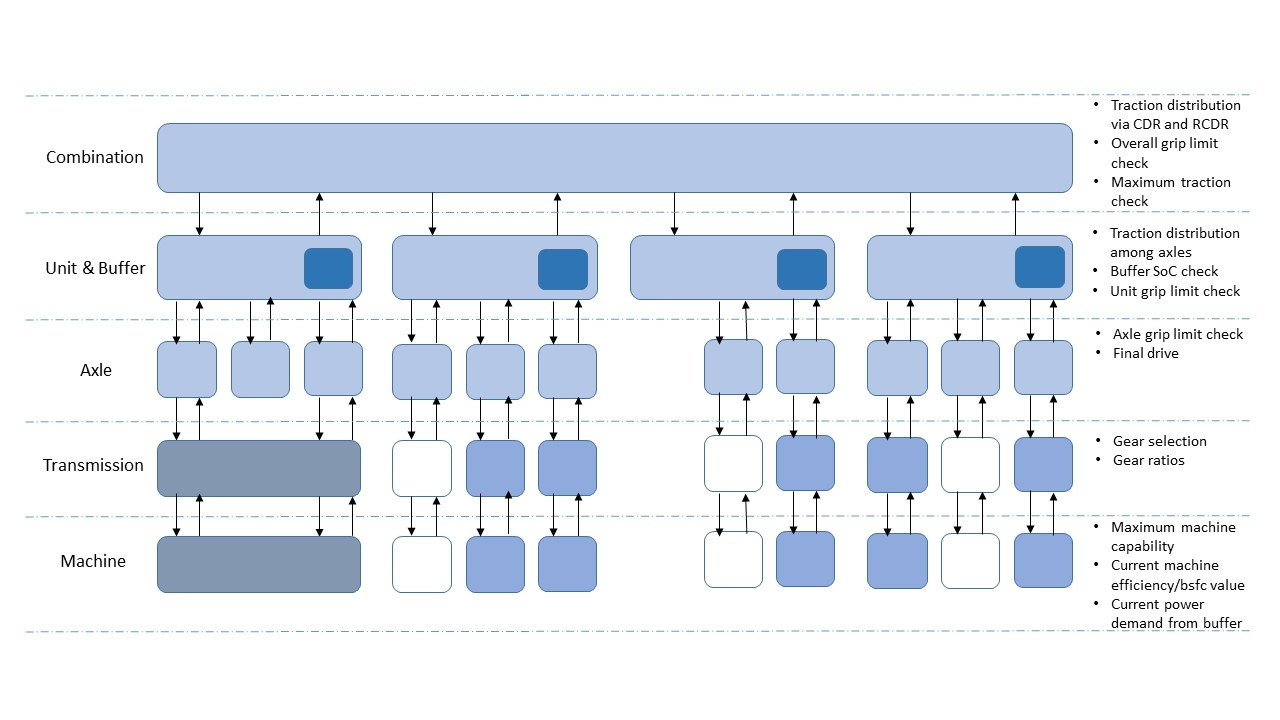
\includegraphics[width=0.75\textwidth]{figures/VehicleModel/vehiclelayout.jpg}
	\end{center}
	\caption{Vehicle model - Structure}
	\label{fig:vehiclelayout}
\end{figure}

\subsection{Combination}\label{sec:combinationstructure}
The truck is constructed using the genetic chromosome as a blueprint as mentioned in Section (??). The units, axles, buffers and axles associated to these units, and the subsequent machines and transmissions associated to these axles and buffers are constructed setting up structure of the combination.The combination level which dictates the overall layout of the truck encapsulates the functionality for the driver model and energy management strategy (EMS).

\begin{figure}
	\begin{center}
		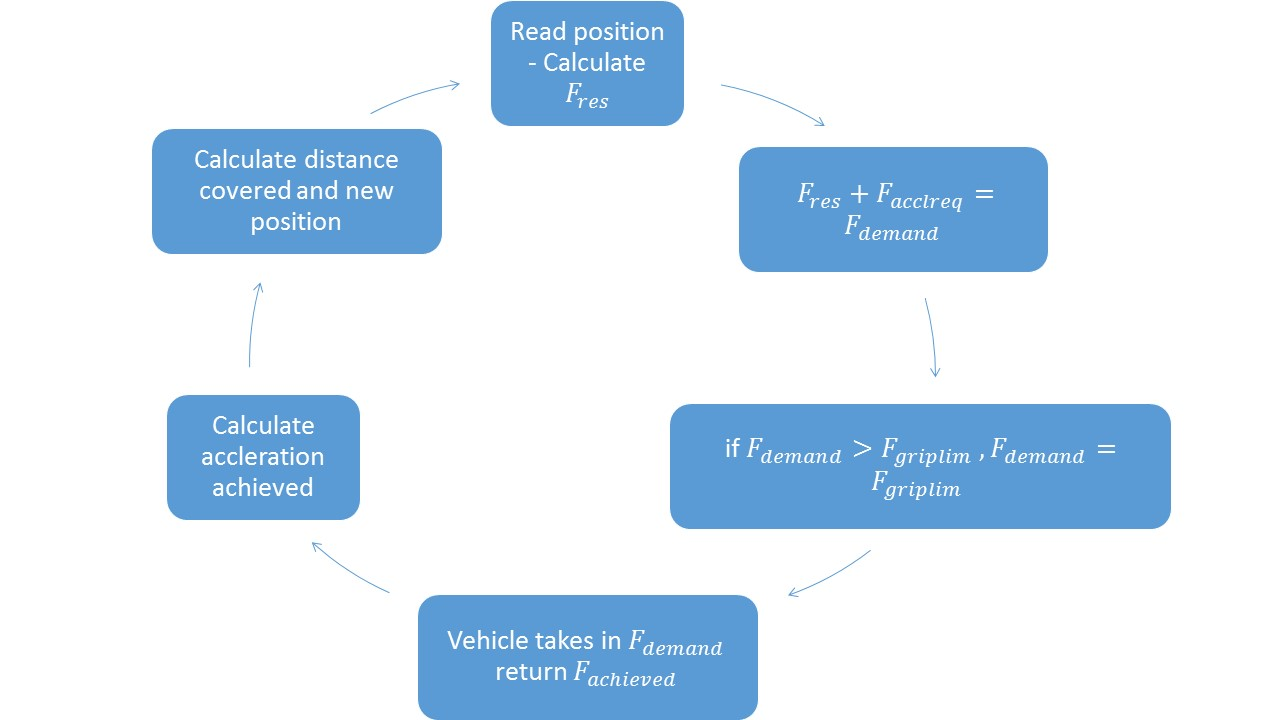
\includegraphics[width=0.75\textwidth]{figures/VehicleModel/combinationfunction.jpg}
	\end{center}
	\caption{Combination functionality}
	\label{fig:combinationfunction}
\end{figure}

\subsection{Units}\label{sec:unitstructure}
The overall truck combination are represented as a collection of 4 units- the tractor, first semi-trailer, dolly and the second semitrailer. The properties that are associated to the units and which vary between them are the overall units load, the battery or fuel tank associated to the units, total number of axles and the number of driven axles. Each unit may have between 2 or 3 associated axles as can be seen in the 3rd layer of the figure (\ref{fig:vehiclelayout}). 

\subsection{Axles}\label{sec:axlestructure}
The individual axle loads are defined for each axle which provides information on the tractive capabilities of that axle through a check for grip limitation. Each axle is either non-driven or is linked to a transmission and through it, a machine, which may either be a motor or an engine in the case of the tractor unit axles. The axle block also contains information on the radius of the tire on the axle and the value of the final drive ratio associated with the axle differential which is used as in equations (\ref{eq:axlespeedgearing}) and (\ref{eq:axletorquegearing}).

\subsection{Transmission}\label{sec:transtructure}
The transmission linked to the axles possess the same structure regardless of the machine. The only property that varies is in fact the number of gears. The other properties are the gear ratios and gear inertias. The functionality of this section is covered by equations (\ref{eq:transpeedgearing}) and (\ref{eq:transtorquegearing})

\subsection{Machines}\label{sec:machinestructure}
The machines, as mentioned earlier maybe either an electric motor or an engine. The machine block contains information about the engine or motor map i.e the maximum torque the machine can produce across the range of operating speed and the b.s.f.c. values and efficiency values associated with each operating point for the engine and motor respectively.  

\subsection{Buffers} \label{sec:bufferstructure}
The buffers associated to the machines are a fuel tank in the case of an engine and a battery when the machine is an electric motor. They are provided with information of the power demand along with the electric machine efficiency or the brake specific fuel consumption of the engine for that operation point of that machine respectively.  
The properties associated with the battery are the current state of charge (SoC) , the total battery capacity and open circuit voltage. The SoC of the battery plays a vital role in determining the torque request to the associated motors as it is essential that the SoC is kept within safe limits of operation. This will be explained in more detail in Section % \ref{sec:ems}

\section{Energy Management Strategy}
The key function of the energy management strategy is to assess the tractive force demand $(F_{dem})$ for that instant and based on certain fixed rules determine the tractive force to be assigned to the 4 units. As mentioned in the earlier section the demand force is a sum of the road resistive forces and the demanded acceleration force. With the instantaneous wheel speed data this demand force is used to calculate a demand power$(P_{dem})$ which may be positive if propulsion is needed or negative which can only mean that some braking is required. 
The logic now splits based on whether it’s in propulsion mode or regenerative mode. When $F_{dem}$ is positive it is checked to see its value is less than the maximum tractive force capacity of all the units put together$(F_{maxtotal})$. If not then the units are assigned to run at their respective maximum traction capability. If it is within range however the idea is to then run the tractor engine at its optimal operating point which produces a traction $F_{engopt}$ which is explained is greater detail below in Section %\ref{sec:oop}%. The trailing units are left to produce the remaining traction and if however the trailing unit traction$(F_trailunit)$ is lower than the grip limited tractive force then the units are set to produce what maximum grip limited force they can pushing the tractor engine to take on the rest.
When the units are able to produce the required force though the question arises on how exactly to divide the force between the trailing units. This functionality was achieved through the introduction of a Traction Distribution Ratio $(TDR)$ which will be explained in greater detail in Section %\ref{sec:tdr}%. 

\begin{figure}
	\begin{center}
		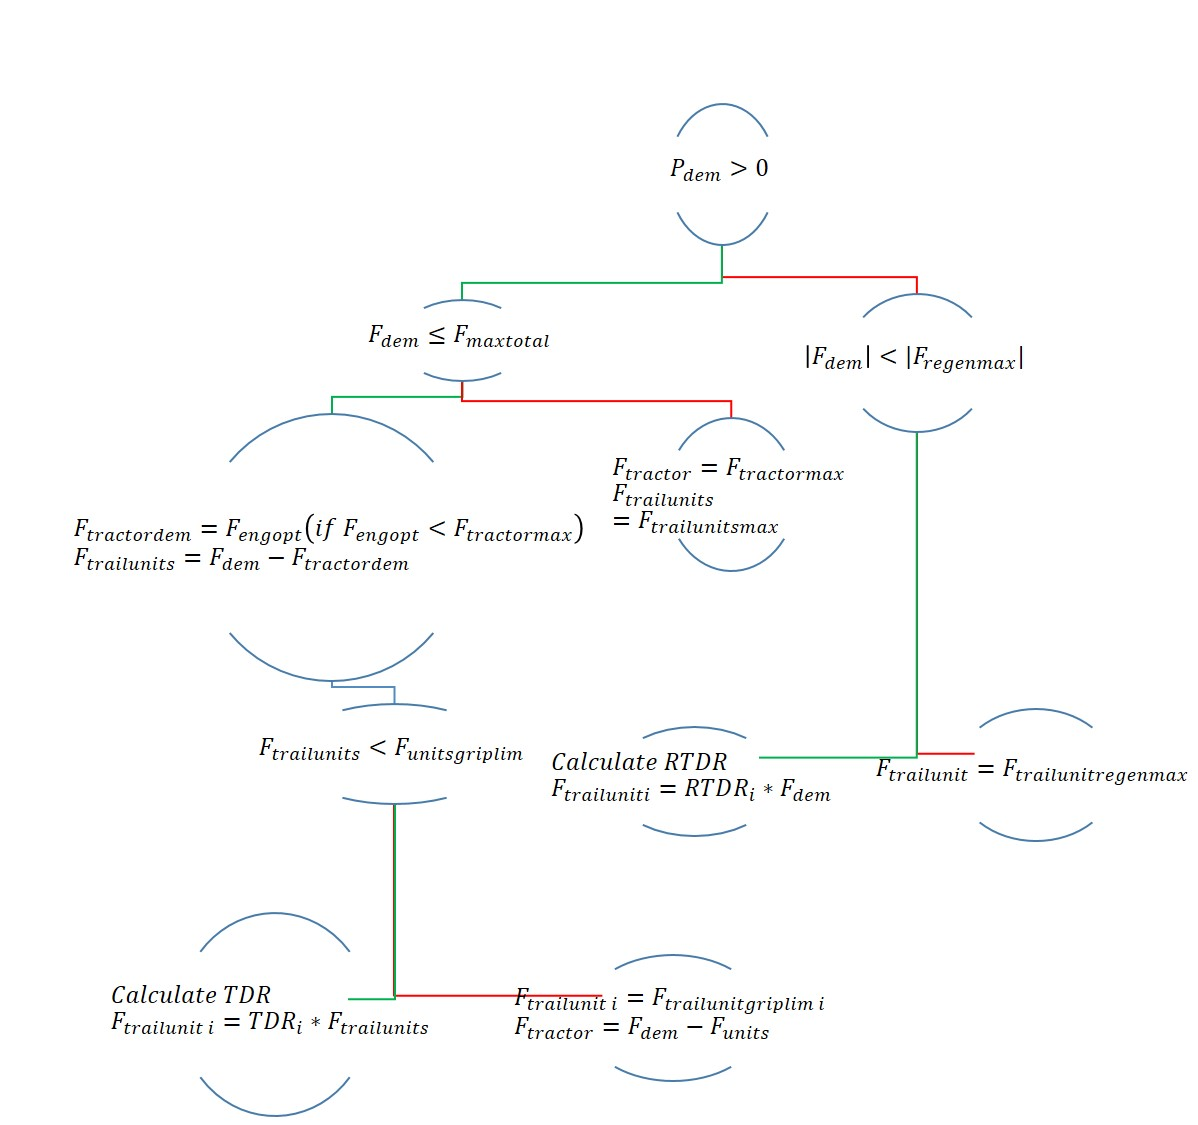
\includegraphics[width=0.75\textwidth]{figures/VehicleModel/ems.jpg}
	\end{center}
	\caption{Heuristic energy management strategy}
	\label{fig:ems}
\end{figure}
	
As can be seen in fig (\ref{fig:ems}) during regeneration mode the logic flows similarly. If magnitude of the traction request is greater than the magnitude of the maximum traction the units can provide for that instant the negative torque requests to the units are limited to their respective maximum regenerative tractive capability$(F_{trailunitregenmax})$. If it is within range however a similar term called Regenerative Traction Distribution Ratio $(RTDR)$ is calculated as explained below.

\subsection{Optimal operating point (OOP)} \label{sec:oop}
The optimal operating point is a set point of operation of an engine at a particular speed and torque at which the engine is the most efficient i.e. the amount of fuel consumed $(m_f)$ per unit brake power$(P_b)$ produced is the lowest as compared to any other point of operation. This term is known as the brake specific fuel consumption $(bsfc)$ as shown below:

\begin{equation} \label{eq:bsfc}
bsfc=\frac{m_f}{P_b}
\end{equation}
 
The point of lowest bsfc for a D16 engine may be seen in fig(\ref{fig:enginemap}) where the blue line describes the maximum level of brake torque that can be produced at each speed of operation.The engine is allowed to operate at this point if possible. That is to say if the amount of torque that is produced at the OOP is sufficient or if the remaining torque can be handled by the electric powertrain. 

\begin{figure}
	\begin{center}
		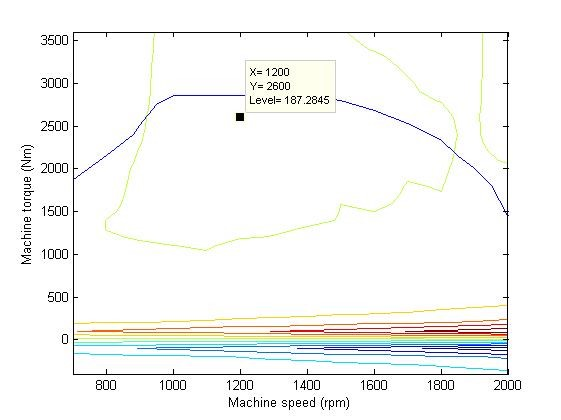
\includegraphics[width=0.75\textwidth]{figures/VehicleModel/enginemap.jpg}
	\end{center}
	\caption{Optimal operating point of a D16 engine}
	\label{fig:enginemap}
\end{figure}

\subsection{Traction distribution ratio (TDR)} \label{sec:tdr}
When a traction request needs to be divided between the trailing units, there are a few factors involved which prevent it from simply being split 3 ways. For example one of the units may have more driven axles than the other hence can offer more traction, the motors driving the units axle may differ with one with one being able to produce more power than the other or one unit’s battery may be close to depleting completely which should prompt low or no traction demand from that unit. In order to address these issues each axle is assigned a TDR which is a ratio of the power availability of each unit over the total power availability as shown in equation (\ref{eq:tdr1}). This means that the summation of all TDRs for all the units add up to 1 thus ensuring that all the required tractive demand is completely assigned if possible. 

\begin{equation} \label{eq:tdr1}
TDR_{unit i}=\frac{(Power Availability)_{unit i}}{Total Power Availability}
\end{equation}
 
\begin{equation} \label{eq:tdr2}
Total Power Availability = \Sigma Power Availability_{unit}
\end{equation}

The power availability term is defined for each unit as a product of Buffer Availability Ratio $(BAR)$ along with the total maximum tractive power that can be produced in that instant by all the electric motors on that unit as shown in equation (\ref{eq:poweravail}). The power term here allows for the unit with the higher power capacity to be assigned with the higher traction.

\begin{equation} \label{eq:poweravail}
Power Availability_{unit} = (BAR)_{unit} * Maximum Tractive Power_{unit i}
\end{equation}
   
The $BAR$ is defined as in equation (\ref{eq:poweravail}) and its value varies between 0 and 1. The lower the value, the lower is the current state of charge level of the buffer on the unit in question. This means that whenever a unit is almost discharged (low $BAR$), the traction assigned to the axles of that unit is lower. 

\begin{equation} \label{eq:bar}
BAR = \frac{SoC_{current}-SoC_{min}}{SoC_{max}-SoC_{min}}
\end{equation}

\subsection{Predictive Control} \label{sec:predcontrol}

\end{document}